% !TEX program = xelatex
\documentclass[9pt, aspectratio=169]{beamer}
\usetheme{metropolis}
\usefonttheme{professionalfonts}

% --- Modern Font Setup ---
\usepackage[T1]{fontenc}
\usepackage{FiraSans}  % Modern, elegant sans-serif font family
\usepackage[scaled=0.95]{FiraMono}  % Matching monospace font

% Lighter, more refined font weights
\renewcommand{\seriesdefault}{l}  % Light weight as default
\renewcommand{\bfseries}{\fontseries{sb}\selectfont}  % Semi-bold instead of bold

% Custom font sizing - more refined
\setbeamerfont{title}{size=\Large, series=\fontseries{m}\selectfont}
\setbeamerfont{subtitle}{size=\normalsize, series=\fontseries{l}\selectfont}
\setbeamerfont{author}{size=\small, series=\fontseries{l}\selectfont}
\setbeamerfont{date}{size=\small, series=\fontseries{l}\selectfont}
\setbeamerfont{frametitle}{size=\normalsize, series=\fontseries{m}\selectfont}
\setbeamerfont{framesubtitle}{size=\footnotesize, series=\fontseries{l}\selectfont}
\setbeamerfont{block title}{size=\normalsize, series=\fontseries{m}\selectfont}
\setbeamerfont{block body}{size=\small}
\setbeamerfont{itemize/enumerate body}{size=\small}
\setbeamerfont{itemize/enumerate subbody}{size=\footnotesize}
\setbeamerfont{section in toc}{size=\normalsize, series=\fontseries{m}\selectfont}
\setbeamerfont{section title}{size=\Large, series=\fontseries{m}\selectfont}

% --- Color Definitions ---
% Primary Theme Colors
\definecolor{PrimaryColor}{RGB}{33,52,72}         % Deep navy
\definecolor{SecondaryColor}{RGB}{84,119,146}     % Desaturated blue-gray
\definecolor{AccentColor}{RGB}{100,156,165}       % Soft steel blue
\definecolor{black}{RGB}{0,0,0}
\definecolor{BackgroundColor}{RGB}{245,247,250}   % Very light cool gray/blue-tinted white
\definecolor{TextColor}{RGB}{40,55,70}            % Darker, cool-toned charcoal
\definecolor{LightGray}{RGB}{220,225,230}         % Soft, cool light gray
\definecolor{DarkGray}{RGB}{70,90,105}            % Cool-toned dark gray

% --- Theme Customization ---
\setbeamercolor{background canvas}{bg=BackgroundColor}
\setbeamercolor{normal text}{fg=TextColor}
\setbeamercolor{frametitle}{bg=PrimaryColor, fg=white}
\setbeamercolor{section in toc}{fg=PrimaryColor}
\setbeamercolor{block title}{bg=PrimaryColor!80, fg=white}
\setbeamercolor{block body}{bg=PrimaryColor!10}
\setbeamercolor{alerted text}{fg=AccentColor}
\setbeamercolor{itemize item}{fg=PrimaryColor}
\setbeamercolor{itemize subitem}{fg=SecondaryColor}

% Progress bar
\setbeamercolor{progress bar}{fg=AccentColor, bg=LightGray}

% --- Packages ---
\usepackage[utf8]{inputenc}
\usepackage{url}
\usepackage{booktabs}
\usepackage{amsmath, amssymb, amsfonts}
\usepackage{fontawesome5}
\usepackage{pifont}
\usepackage[most]{tcolorbox}
\tcbuselibrary{skins, listings}
\usepackage{colortbl}
\usepackage{array}
\usepackage{adjustbox}
\usepackage{ragged2e}

% --- Packages for plotting discrete and continuous signals and spectrums ---
\usepackage{tikz}
\usepackage{circuitikz} % Useful for signal processing block diagrams
\usepackage{pgfplots}
\usepackage{graphicx}
\usepackage{caption}
\usepackage{subcaption}

\usetikzlibrary{shapes.callouts, positioning, arrows.meta, shapes.geometric, shadows, calc, patterns, backgrounds, shadings, fit, chains, decorations.pathreplacing, intersections}
\usepgfplotslibrary{fillbetween}
\usepgfplotslibrary{polar}
\pgfplotsset{compat=1.18}
\pgfplotsset{
    plot coordinates/math parser=false,
    signal/.style={thick, color=PrimaryColor},
    spectrum/.style={thick, color=AccentColor},
    discrete/.style={ycomb, mark=*, mark options={fill=white, draw=PrimaryColor}, color=PrimaryColor, thick},
}

% --- Custom Commands ---
\newcommand{\cmark}{\textcolor{PrimaryColor}{\ding{51}}}
\newcommand{\xmark}{\textcolor{AccentColor}{\ding{55}}}
\newcommand{\highlight}[1]{\textcolor{PrimaryColor}{\textbf{#1}}}

% --- Custom tcolorbox environments ---
\newtcolorbox{conceptbox}[1]{
    colback=PrimaryColor!10,
    colframe=PrimaryColor,
    title=#1,
    fonttitle=\small\bfseries,
    fontupper=\small,
    rounded corners
}

\newtcolorbox{insightbox}[1]{
    colback=AccentColor!10,
    colframe=AccentColor,
    title=#1,
    fonttitle=\small\bfseries,
    fontupper=\small,
    rounded corners
}

\newtcolorbox{algorithmbox}[1]{
    colback=SecondaryColor!10,
    colframe=SecondaryColor,
    title=#1,
    fonttitle=\small\bfseries,
    fontupper=\small,
    rounded corners
}

\newtcblisting{codelistingbox}[2][]{
    colback=SecondaryColor!10,
    colframe=SecondaryColor,
    title=#2,
    fonttitle=\small\bfseries,
    rounded corners,
    listing only,
    listing options={
            language=#1,
            basicstyle=\ttfamily\footnotesize,
            keywordstyle=\color{PrimaryColor}\bfseries,
            commentstyle=\color{SecondaryColor}\itshape,
            stringstyle=\color{AccentColor},
            numbers=left,
            numberstyle=\tiny\color{DarkGray},
            stepnumber=1,
            showstringspaces=false,
            tabsize=4
        }
}


\subtitle{Signals and Linear Systems}
\date{}
\author{Ashrafur Rahman\\Lecturer, CSE, BUET}
\institute{ashrafur@cse.buet.ac.bd}


\title{More Laplace Transform}

\begin{document}

\pgfplotsset{every axis/.append style={tick style={draw=none}}}

\maketitle

\begin{frame}{Outline}
  \begin{itemize}
    \item \textbf{Properties of the Laplace Transform}
      \begin{itemize}
        \item Algebraic rules, ROC behavior, and quick examples
        \item A compact summary table
      \end{itemize}
    \item \textbf{Some Laplace Transform Pairs}
      \begin{itemize}
        \item Common right-sided, left-sided, and oscillatory signals
      \end{itemize}
    \item \textbf{Analysis and Characterization of LTI Systems Using LT}
      \begin{itemize}
        \item System function, causality, and stability
      \end{itemize}
    \item \textbf{Differential Equations and System Models}
      \begin{itemize}
        \item Converting differential equations into algebra
        \item Solving a zero-state response and analyzing an RLC circuit
      \end{itemize}
  \end{itemize}
\end{frame}

\section{Properties of the Laplace Transform}

\begin{frame}[t]{Linearity}
  \small
  \begin{conceptbox}{Linearity}
    If $x_1(t) \stackrel{\mathcal{L}}{\longleftrightarrow} X_1(s)$ with ROC $R_1$ and
    $x_2(t) \stackrel{\mathcal{L}}{\longleftrightarrow} X_2(s)$ with ROC $R_2$, then
    \[
      a x_1(t) + b x_2(t) \stackrel{\mathcal{L}}{\longleftrightarrow} a X_1(s) + b X_2(s)
    \]
    with ROC containing at least $R_1 \cap R_2$.
  \end{conceptbox}

  \vspace{0.06cm}
  \textit{Proof sketch:}
  \[
    \mathcal{L}\{a x_1(t)+b x_2(t)\}=a\int_{0}^{\infty} e^{-st} x_1(t) dt + b\int_{0}^{\infty} e^{-st} x_2(t) dt =aX_1(s)+bX_2(s)
  \]
  so convergence is guaranteed wherever both original transforms converge.

  \vspace{0.08cm}
  \textbf{Example}
  \[
    x(t)=e^{-t}u(t)+2e^{-2t}u(t)
    \stackrel{\mathcal{L}}{\longleftrightarrow}
    \frac{1}{s+1}+\frac{2}{s+2},
    \qquad \text{Re}\{s\}>-1
  \]

  \vspace{0.08cm}
  \begin{insightbox}{Important caution}
    The intersection ROC is a guaranteed starting point, not always the final answer.
  \end{insightbox}
\end{frame}

\begin{frame}[t]{Example 9.13: Cancellation Can Extend the ROC}
  \small
  \begin{columns}[T]
    \begin{column}{0.52\textwidth}
    \begin{itemize}\setlength{\itemsep}{0.2em}
        \item Let
          \[
            X_1(s)=\frac{1}{s+1},
            \qquad \text{Re}\{s\}>-1
          \]
          and
          \[
            X_2(s)=\frac{1}{(s+1)(s+2)},
            \qquad \text{Re}\{s\}>-1
          \]
        \item By linearity, the ROC of $X_1(s)-X_2(s)$ must contain at least
          \[
            \text{Re}\{s\}>-1
          \]
        \item Form the difference:
          \[
            X(s)=X_1(s)-X_2(s)
            =\frac{1}{s+1}-\frac{1}{(s+1)(s+2)}
            =\frac{1}{s+2}
          \]
        \item The pole at $s=-1$ disappears after cancellation, so the actual ROC expands to
          \[
            \text{Re}\{s\}>-2
          \]
      \end{itemize}
      \textbf{Takeaway:} the intersection ROC is only the guaranteed part.
      If poles cancel, the actual ROC can extend further.
    \end{column}
    \begin{column}{0.48\textwidth}
      \begin{center}
        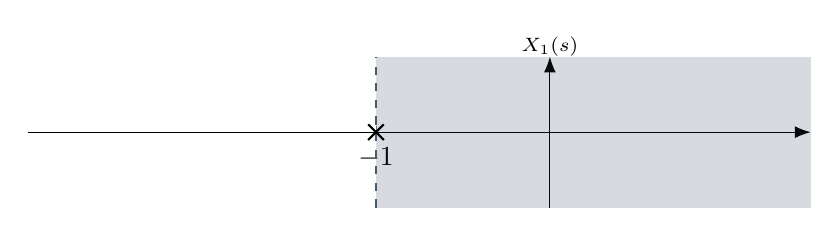
\begin{tikzpicture}
          \begin{axis}[
              width=0.95\textwidth, height=3.5cm,
              axis lines=middle, axis line style={-{Latex[length=2mm]}},
              xmin=-3, xmax=1.5, ymin=-1.5, ymax=1.5,
              xtick={-1}, xticklabels={$-1$}, ytick=\empty,
              clip=false
            ]
            \fill[PrimaryColor, fill opacity=0.18] (axis cs:-1,-1.5) rectangle (axis cs:1.5,1.5);
            \draw[dashed, thick, DarkGray] (axis cs:-1,-1.5) -- (axis cs:-1,1.5);
            \addplot[only marks, mark=x, mark options={scale=2, thick}] coordinates {(-1,0)};
            \node at (axis cs:0,1.7) {\scriptsize $X_1(s)$};
          \end{axis}
        \end{tikzpicture}

        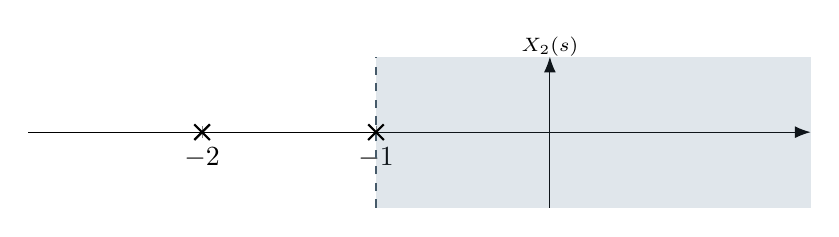
\begin{tikzpicture}
          \begin{axis}[
              width=0.95\textwidth, height=3.5cm,
              axis lines=middle, axis line style={-{Latex[length=2mm]}},
              xmin=-3, xmax=1.5, ymin=-1.5, ymax=1.5,
              xtick={-2,-1}, xticklabels={$-2$,$-1$}, ytick=\empty,
              clip=false
            ]
            \fill[SecondaryColor, fill opacity=0.18] (axis cs:-1,-1.5) rectangle (axis cs:1.5,1.5);
            \draw[dashed, thick, DarkGray] (axis cs:-1,-1.5) -- (axis cs:-1,1.5);
            \addplot[only marks, mark=x, mark options={scale=2, thick}] coordinates {(-2,0) (-1,0)};
            \node at (axis cs:0,1.7) {\scriptsize $X_2(s)$};
          \end{axis}
        \end{tikzpicture}

        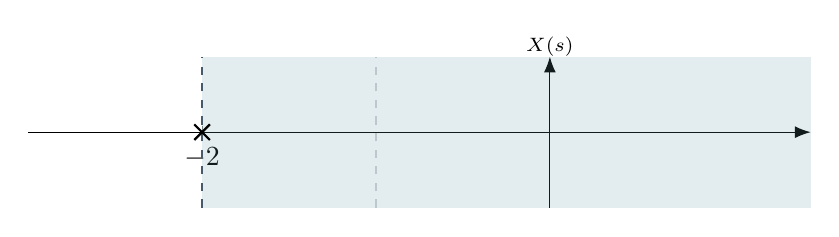
\begin{tikzpicture}
          \begin{axis}[
              width=0.95\textwidth, height=3.5cm,
              axis lines=middle, axis line style={-{Latex[length=2mm]}},
              xmin=-3, xmax=1.5, ymin=-1.5, ymax=1.5,
              xtick={-2}, xticklabels={$-2$}, ytick=\empty,
              clip=false
            ]
            \fill[AccentColor, fill opacity=0.18] (axis cs:-2,-1.5) rectangle (axis cs:1.5,1.5);
            \draw[dashed, thick, DarkGray] (axis cs:-2,-1.5) -- (axis cs:-2,1.5);
            \addplot[only marks, mark=x, mark options={scale=2, thick}] coordinates {(-2,0)};
            \draw[dashed, thick, DarkGray, opacity=0.25] (axis cs:-1,-1.5) -- (axis cs:-1,1.5);
            \node at (axis cs:0,1.7) {\scriptsize $X(s)$};
          \end{axis}
        \end{tikzpicture}
      \end{center}
    \end{column}
  \end{columns}
\end{frame}

\begin{frame}[t]{Time Shifting}
  \small
  \begin{columns}[T]
    \begin{column}{0.53\textwidth}
      \footnotesize
      \begin{conceptbox}{Time Shifting}
        \[
          x(t-t_0) \stackrel{\mathcal{L}}{\longleftrightarrow} e^{-st_0} X(s),
          \qquad \text{ROC} = R
        \]
      \end{conceptbox}

      \vspace{0.08cm}
      \textit{Proof sketch:}
      Using the substitution $\tau = t-t_0$,
      \begin{align*}
        \mathcal{L}\{x(t-t_0)\}
        & = \int_{-\infty}^{\infty} x(t-t_0) e^{-st} dt \\
        & = \int_{-\infty}^{\infty} x(\tau) e^{-s(\tau+t_0)} d\tau \\
        & = e^{-st_0} \int_{-\infty}^{\infty} x(\tau) e^{-s\tau} d\tau \\
        & = e^{-st_0} X(s)
      \end{align*}

      \vspace{0.15cm}
      \textbf{Example}
      \[
        u(t-2) \stackrel{\mathcal{L}}{\longleftrightarrow} \frac{e^{-2s}}{s},
        \qquad \text{Re}\{s\}>0
      \]

      \vspace{0.1cm}
      \textit{The delay changes the transform, not the ROC.}
    \end{column}
    \begin{column}{0.47\textwidth}
      \begin{center}
        \vspace{2cm}
        \begin{tikzpicture}
          \begin{axis}[
              width=0.96\textwidth, height=3.4cm,
              axis lines=middle, axis line style={-{Latex[length=2mm]}},
              xmin=-0.5, xmax=4.2, ymin=-0.1, ymax=1.4,
              xtick={0,2}, xticklabels={$0$,$2$},
              ytick={1}, yticklabels={$1$},
              xlabel={$t$}, ylabel={$x(t)$},
              xlabel style={anchor=west, at={(axis cs:4.25,0)}},
              ylabel style={anchor=south, at={(axis cs:0,1.45)}},
              clip=false
            ]
            \draw[thick, SecondaryColor!50] (axis cs:-0.5,0) -- (axis cs:0,0) -- (axis cs:0,1) -- (axis cs:2,1) -- (axis cs:2,0);
            \draw[thick, PrimaryColor] (axis cs:0,0) -- (axis cs:2,0) -- (axis cs:2,1) -- (axis cs:4.2,1);
            \draw[dashed, DarkGray] (axis cs:2,0) -- (axis cs:2,1);
            \node[SecondaryColor, above] at (axis cs:1,1.05) {\scriptsize $u(t)$};
            \node[PrimaryColor, above] at (axis cs:3.15,1.05) {\scriptsize $u(t-2)$};
          \end{axis}
        \end{tikzpicture}
      \end{center}
    \end{column}
  \end{columns}
\end{frame}

\begin{frame}[t]{Shifting in the \texorpdfstring{$s$}{s}-Domain}
  \begin{columns}[T]
    \begin{column}{0.55\textwidth}
      \footnotesize
      \vspace{-0.2cm}
      \begin{conceptbox}{Shifting in the $s$-Domain}
        If $x(t) \stackrel{\mathcal{L}}{\longleftrightarrow} X(s)$ with ROC $R$, then
        \[
          e^{s_0 t}x(t) \stackrel{\mathcal{L}}{\longleftrightarrow} X(s-s_0)
        \]
        with $\text{ROC} = R + \text{Re}\{s_0\}$.
      \end{conceptbox}

      \textit{Proof sketch:} \\

      Using the substitution $s' = s - s_0$,
      \begin{align*}
        \mathcal{L}\{e^{s_0 t}x(t)\}&=\int_{-\infty}^{\infty} e^{s_0 t} x(t) e^{-st} dt \\
        &= \int_{-\infty}^{\infty} x(t) e^{-s' t} dt \\
        &= X(s') = X(s-s_0)
      \end{align*}

      so the ROC becomes $R + \text{Re}\{s_0\}$ (right shifted by $\text{Re}\{s_0\}$).

      \vspace{0.1cm}
      \textbf{Example:} from $u(t) \stackrel{\mathcal{L}}{\longleftrightarrow} \frac{1}{s}$,
      \[
        e^{-2t}u(t) \stackrel{\mathcal{L}}{\longleftrightarrow} \frac{1}{s+2},
        \qquad \text{Re}\{s\}>-2
      \]
    \end{column}
    \begin{column}{0.45\textwidth}
      \textbf{ROC Shift}\\[0.1cm]
      \begin{center}
        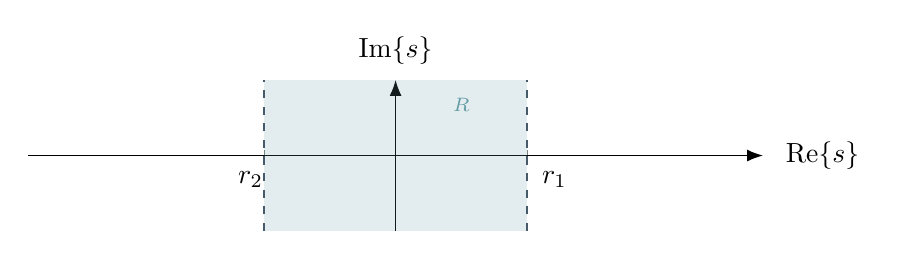
\begin{tikzpicture}
          \begin{axis}[
              width=0.9\textwidth, height=3.5cm,
              axis lines=middle, axis line style={-{Latex[length=2mm]}},
              xmin=-2.8, xmax=2.8, ymin=-2.0, ymax=2.0,
              xtick={-1,1}, xticklabels={$r_2 \quad$,$\qquad r_1$},
              ytick=\empty,
              xlabel={$\text{Re}\{s\}$},
              ylabel={$\text{Im}\{s\}$},
              xlabel style={anchor=west, at={(axis cs:2.9,0)}},
              ylabel style={anchor=south, at={(axis cs:0,2.15)}},
              clip=false
            ]
            \fill[AccentColor, fill opacity=0.18] (axis cs:-1,-2) rectangle (axis cs:1,2);
            \draw[dashed, thick, DarkGray] (axis cs:-1,-2) -- (axis cs:-1,2);
            \draw[dashed, thick, DarkGray] (axis cs:1,-2) -- (axis cs:1,2);
            \node[AccentColor] at (axis cs:0.5,1.35) {\scriptsize $R$};
          \end{axis}
        \end{tikzpicture}

        \vspace{0.05cm}
        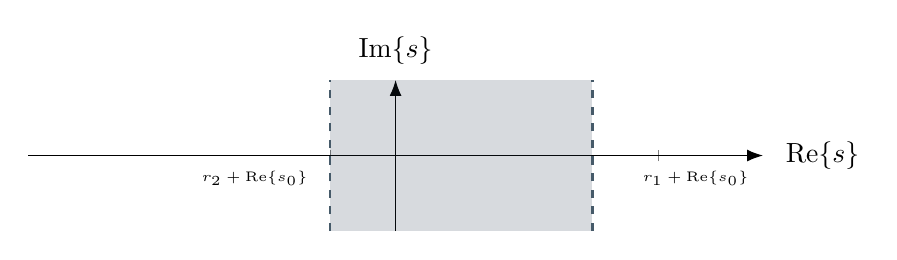
\begin{tikzpicture}
          \begin{axis}[
              width=0.9\textwidth, height=3.5cm,
              axis lines=middle, axis line style={-{Latex[length=2mm]}},
              xmin=-2.8, xmax=2.8, ymin=-2.0, ymax=2.0,
              xtick={-0.5,2}, xticklabels={$r_2+\text{Re}\{s_0\}\qquad\qquad\qquad\qquad$,$\qquad\qquad r_1+\text{Re}\{s_0\}$},
              xticklabel style={font=\tiny},
              ytick=\empty,
              xlabel={$\text{Re}\{s\}$},
              ylabel={$\text{Im}\{s\}$},
              xlabel style={anchor=west, at={(axis cs:2.9,0)}},
              ylabel style={anchor=south, at={(axis cs:0,2.15)}},
              clip=false
            ]
            \fill[PrimaryColor, fill opacity=0.18] (axis cs:-0.5,-2) rectangle (axis cs:1.5,2);
            \draw[dashed, thick, DarkGray] (axis cs:-0.5,-2) -- (axis cs:-0.5,2);
            \draw[dashed, thick, DarkGray] (axis cs:1.5,-2) -- (axis cs:1.5,2);
            % \node[PrimaryColor] at (axis cs:1,1.35) {\scriptsize $R+\text{Re}\{s_0\}$};
          \end{axis}
        \end{tikzpicture}
      \end{center}
    \end{column}
  \end{columns}
\end{frame}

\begin{frame}[t]{Time Scaling}
  \small
  \vspace{-0.4cm}
  \begin{columns}[T]
    \begin{column}{0.53\textwidth}
      \footnotesize
      \begin{conceptbox}{Time Scaling}
        \[
          x(at) \stackrel{\mathcal{L}}{\longleftrightarrow} \frac{1}{|a|}X\!\left(\frac{s}{a}\right)
        \]
        with $\text{ROC} = aR$.
      \end{conceptbox}
      \vspace{0.2cm}
      \textit{Proof sketch:} Let $\lambda = at$, so $dt = d\lambda / a$.
      \begin{align*}
        \mathcal{L}\{x(at)\}
        & = \int_{-\infty}^{\infty} x(at) e^{-st} dt \\
        &= \int_{-\infty}^{\infty} x(\lambda) e^{-s\lambda/a} \frac{d\lambda}{a} \\
        & =
        \begin{cases}
          \frac{1}{a}\int_{-\infty}^{\infty} x(\lambda) e^{-\lambda(s/a)} d\lambda = \frac{1}{a} X\!\left(\frac{s}{a}\right), & a>0 \\
          \frac{1}{a}\int_{\infty}^{-\infty} x(\lambda) e^{-\lambda(s/a)} d\lambda = -\frac{1}{a} X\!\left(\frac{s}{a}\right), & a<0
        \end{cases} \\
        & = \frac{1}{|a|} X\!\left(\frac{s}{a}\right)
      \end{align*}

      Note that:
      \begin{itemize}
          \scriptsize
        \item If $0<a<1$, the signal is compressed in time.
        \item If $a>1$, the signal is stretched in time.
        \item If $a<0$, the signal is flipped in time and scaled.
      \end{itemize}
    \end{column}
    \begin{column}{0.47\textwidth}
      \vspace{0.5cm}
      \textbf{Scaling example:}
      \[
        x(t)=e^{-t}u(t) \Longrightarrow X(s)=\frac{1}{s+1}
      \]
      Hence,
      \[
        x(2t)=e^{-2t}u(t)
        \stackrel{\mathcal{L}}{\longleftrightarrow}
        \frac{1}{2}X\!\left(\frac{s}{2}\right)
        = \frac{1}{s+2}
      \]

      \textbf{ROC Under Scaling} \\[0.05cm]
      \begin{center}
        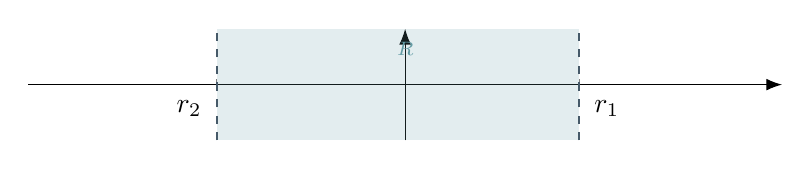
\begin{tikzpicture}
          \begin{axis}[
              width=0.92\textwidth, height=3cm,
              axis lines=middle, axis line style={-{Latex[length=2mm]}},
              xmin=-2.6, xmax=2.6, ymin=-1.7, ymax=1.7,
              xtick={-1.3,1.2}, xticklabels={$r_2\qquad$,$\qquad r_1$},
              ytick=\empty, clip=false
            ]
            \fill[AccentColor, fill opacity=0.18] (axis cs:-1.3,-1.7) rectangle (axis cs:1.2,1.7);
            \draw[dashed, thick, DarkGray] (axis cs:-1.3,-1.7) -- (axis cs:-1.3,1.7);
            \draw[dashed, thick, DarkGray] (axis cs:1.2,-1.7) -- (axis cs:1.2,1.7);
            \node[AccentColor] at (axis cs:0,1.1) {\scriptsize $R$};
          \end{axis}
        \end{tikzpicture}

        \vspace{0.05cm}
        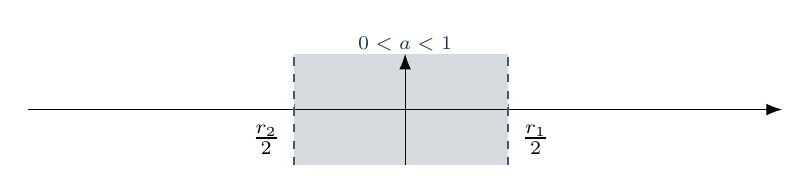
\begin{tikzpicture}
          \begin{axis}[
              width=0.92\textwidth, height=3cm,
              axis lines=middle, axis line style={-{Latex[length=2mm]}},
              xmin=-2.2, xmax=2.2, ymin=-1.7, ymax=1.7,
              xtick={-0.65,0.6}, xticklabels={$\frac{r_2}{2}\qquad$,$\qquad \frac{r_1}{2}$},
              ytick=\empty, clip=false
            ]
            \fill[PrimaryColor, fill opacity=0.18] (axis cs:-0.65,-1.7) rectangle (axis cs:0.6,1.7);
            \draw[dashed, thick, DarkGray] (axis cs:-0.65,-1.7) -- (axis cs:-0.65,1.7);
            \draw[dashed, thick, DarkGray] (axis cs:0.6,-1.7) -- (axis cs:0.6,1.7);
            \node[PrimaryColor] at (axis cs:0,2) {\scriptsize $0<a<1$};
          \end{axis}
        \end{tikzpicture}

        \vspace{0.05cm}
      \end{center}
    \end{column}
  \end{columns}
\end{frame}

\begin{frame}[t]{Time Reversal}
  \begin{columns}[T]
    \begin{column}{0.54\textwidth}
      \begin{conceptbox}{Time Reversal}
        Time reversal is the special case $a=-1$:
        \[
          x(-t) \stackrel{\mathcal{L}}{\longleftrightarrow} X(-s),
          \qquad \text{ROC}=-R
        \]
      \end{conceptbox}

      \vspace{0.1cm}
      \textbf{Example:}
      \[
        e^{-t}u(t)
        \stackrel{\mathcal{L}}{\longleftrightarrow}
        \frac{1}{s+1},
        \qquad \text{Re}\{s\}>-1
      \]
      hence
      \[
        e^{t}u(-t)
        \stackrel{\mathcal{L}}{\longleftrightarrow}
        \frac{1}{1-s},
        \qquad \text{Re}\{s\}<1
      \]
    \end{column}
    \begin{column}{0.46\textwidth}
      \textbf{ROC Flip in the $s$-Plane}\\[0.1cm]
      \begin{center}

        \vspace{0.5cm}

        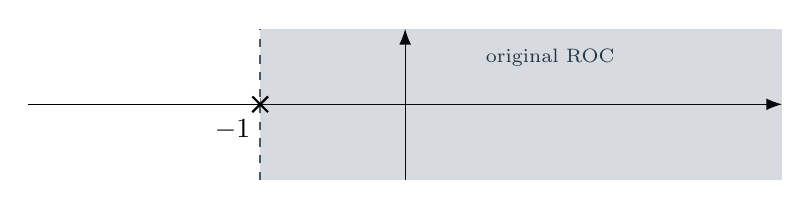
\begin{tikzpicture}
          \begin{axis}[
              width=0.92\textwidth, height=3.5cm,
              axis lines=middle, axis line style={-{Latex[length=2mm]}},
              xmin=-2.6, xmax=2.6, ymin=-1.7, ymax=1.7,
              xtick={-1}, xticklabels={$-1\qquad$},
              ytick=\empty, clip=false
            ]
            \fill[PrimaryColor, fill opacity=0.18] (axis cs:-1,-1.7) rectangle (axis cs:2.6,1.7);
            \draw[dashed, thick, DarkGray] (axis cs:-1,-1.7) -- (axis cs:-1,1.7);
            \addplot[only marks, mark=x, mark options={scale=2, thick}] coordinates {(-1,0)};
            \node[PrimaryColor] at (axis cs:1,1.05) {\scriptsize original ROC};
          \end{axis}
        \end{tikzpicture}

        \vspace{0.5cm}

        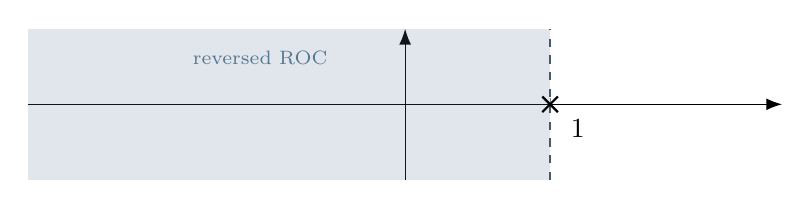
\begin{tikzpicture}
          \begin{axis}[
              width=0.92\textwidth, height=3.5cm,
              axis lines=middle, axis line style={-{Latex[length=2mm]}},
              xmin=-2.6, xmax=2.6, ymin=-1.7, ymax=1.7,
              xtick={1}, xticklabels={$\qquad 1$},
              ytick=\empty, clip=false
            ]
            \fill[SecondaryColor, fill opacity=0.18] (axis cs:-2.6,-1.7) rectangle (axis cs:1,1.7);
            \draw[dashed, thick, DarkGray] (axis cs:1,-1.7) -- (axis cs:1,1.7);
            \addplot[only marks, mark=x, mark options={scale=2, thick}] coordinates {(1,0)};
            \node[SecondaryColor] at (axis cs:-1,1.05) {\scriptsize reversed ROC};
          \end{axis}
        \end{tikzpicture}
      \end{center}
    \end{column}
  \end{columns}
\end{frame}

\begin{frame}[t]{Conjugation}
  \small
  \begin{conceptbox}{Conjugation}
    \begin{align*}
      x^*(t) \stackrel{\mathcal{L}}{\longleftrightarrow} X^*(s^*)
    \end{align*}
    with $\text{ROC}=R$.
  \end{conceptbox}

  \textit{Proof sketch:}
  \begin{align*}
    \mathcal{L}\{x^*(t)\}
    & = \int_{-\infty}^{\infty} x^*(t) e^{-st} dt
    = \left(\int_{-\infty}^{\infty} x(t) e^{-s^* t} dt\right)^*
    = X^*(s^*)
  \end{align*}
  \textbf{Special case:}
  Note $x(t)$ is real, then $x^*(t)=x(t)$, so $X^*(s^*)=X(s)$.
  So, if $X(s) = 0$ or $X(s) = \pm \infty$ at some $s_0$, then $X(s_0^*)$ must also be zero or $\pm \infty$.
  \begin{insightbox}{Pole-Zero Symmetry for Real Signals}
    If $x(t)$ is real and $X(s)$ is rational, its poles and zeros are either real or form complex conjugate pairs.
  \end{insightbox}

  \textbf{Example:} In example 9.4 the transform of real $x(t)$ has poles at $s=1\pm 3j$ that are complex conjugates.
\end{frame}

\begin{frame}[t]{Convolution}
  \footnotesize
  \begin{conceptbox}{Convolution}
    \[
      x_1(t)*x_2(t)
      \stackrel{\mathcal{L}}{\longleftrightarrow}
      X_1(s)X_2(s)
    \]
    with ROC containing at least $R_1\cap R_2$.
  \end{conceptbox}

  \textit{Proof sketch:}
  \begin{align*}
    \mathcal{L}\{x_1(t)*x_2(t)\}
    & = \int_{-\infty}^{\infty} \left(\int_{-\infty}^{\infty} x_1(\tau) x_2(t-\tau) d\tau\right) e^{-st} dt
    = \int_{-\infty}^{\infty} x_1(\tau) \left(\int_{-\infty}^{\infty} x_2(t-\tau) e^{-st} dt\right) d\tau \\
    & = \int_{-\infty}^{\infty} x_1(\tau) e^{-s\tau} d\tau \int_{-\infty}^{\infty} x_2(\lambda) e^{-s\lambda} d\lambda \qquad \text{substituting } \lambda = t - \tau \\
    & = X_1(s) X_2(s), \qquad \text{ROC} \supseteq R_1 \cap R_2 \text{ as both integrals converge in this region}
  \end{align*}

  \begin{insightbox}{Important caution}
    The intersection ROC is only the guaranteed part, not always the final answer.
    If poles cancel, the actual ROC can extend further.
  \end{insightbox}

  \textbf{Example:}\\
  If $X_1(s)=\frac{s+1}{s+2}$ with $\text{Re}\{s\}>-2$ and $X_2(s)=\frac{s+2}{s+1}$
  with $\text{Re}\{s\}>-1$, then $X_1(s)X_2(s)=1$ and ROC is the entire $s$-plane.
\end{frame}

\begin{frame}[t]{Differentiation in Time}
  \footnotesize
  \begin{conceptbox}{Differentiation in Time}
    \[
      \frac{d}{dt}x(t)
      \stackrel{\mathcal{L}}{\longleftrightarrow}
      sX(s)
    \]
    with ROC containing $R$.
  \end{conceptbox}

  \textit{Proof sketch:} Taking the inverse transform,
  \begin{align*}
    x(t) & = \frac{1}{2\pi j} \int_{c-j\infty}^{c+j\infty} X(s) e^{st} ds = \mathcal{L}^{-1}\{X(s)\} \\
    \frac{d}{dt}x(t) & = \frac{1}{2\pi j} \int_{c-j\infty}^{c+j\infty} s X(s) e^{st} ds = \mathcal{L}^{-1}\{sX(s)\}
  \end{align*}
  Therefore,
  \begin{align*}
    \mathcal{L}\left\{\frac{d}{dt}x(t)\right\} = sX(s)
  \end{align*}
  which converges in $R$, so the ROC of the derivative contains $R$.
  \begin{insightbox}{Why it matters}
    Differential equations become algebraic equations because every derivative contributes a factor of $s$.
  \end{insightbox}
\end{frame}

\begin{frame}[t]{Differentiation in Time}
  \small
  \textbf{Example:}
  \begin{align*}
    u(t) & \stackrel{\mathcal{L}}{\longleftrightarrow} \frac{1}{s}, & \text{Re}\{s\}>0 \\
    \frac{d}{dt}u(t)  = \delta(t) & \stackrel{\mathcal{L}}{\longleftrightarrow} s \cdot \frac{1}{s} = 1, & \text{Re}\{s\}>-\infty
  \end{align*}
  \vspace{0.25cm}

  \noindent
  \textbf{Note} again that the ROC of the derivative is larger than that of the original signal.
  $X(s) = \frac{1}{s}$ had a single-order pole at $s=0$, but multiplication with $s$ cancelled the pole.
  \vspace{0.25cm}

  If $X(s)$ has a first-order pole at $s=0$, then multiplication by $s$ cancels the pole, so the ROC of $sX(s)$ extends.

  \begin{insightbox}{Important caution}
    The ROC of the derivative can be larger than that of the original signal.
    If $X(s)$ has a pole at $s=0$, then multiplication by $s$ cancels the pole, so the ROC of $sX(s)$ extends to include $s=0$.
  \end{insightbox}
\end{frame}

\begin{frame}[t]{Differentiation in the \texorpdfstring{$s$}{s}-Domain}
  \small
  \begin{conceptbox}{Differentiation in the $s$-Domain}
    \[
      -t\,x(t)
      \stackrel{\mathcal{L}}{\longleftrightarrow}
      \frac{dX(s)}{ds}
    \]
    with $\text{ROC}=R$.
  \end{conceptbox}
  \vspace{0.5cm}

  \textit{Proof sketch:}
  \[
    \frac{dX(s)}{ds}
    =
    \frac{d}{ds}\int_{-\infty}^{\infty} x(t)e^{-st}dt
    =
    \int_{-\infty}^{\infty} (-t)x(t)e^{-st}dt
    = \mathcal{L}\{-t x(t)\}
  \]
  \begin{itemize}
    \item As for every $s \in R$ differentiation is valid, the ROC contains $R$.
    \item If $\int_{-\infty}^{\infty} |t||x(t)| e^{-\sigma t} dt$ converges for some $\sigma$, then $\int_{-\infty}^{\infty} |x(t)| e^{-\sigma t} dt$ also converges.
  \end{itemize}
  So, the ROC of $\frac{dX(s)}{ds}$ is exactly $R$.

\end{frame}

\begin{frame}[t]{Example 9.14: Differentiation in the \texorpdfstring{$s$}{s}-Domain}

  \textbf{Example:}
  since
  \[
    e^{-at}u(t)
    \stackrel{\mathcal{L}}{\longleftrightarrow}
    \frac{1}{s+a},
    \qquad \text{Re}\{s\}>-a
  \]
  we get
  \[
    t e^{-at}u(t)
    \stackrel{\mathcal{L}}{\longleftrightarrow}
    -\frac{d}{ds} \left( \frac{1}{s+a} \right) =  \frac{1}{(s+a)^2},
    \qquad \text{Re}\{s\}>-a
  \]
  We can continue to differentiate to get,
  \[
    \frac{t^2}{2} e^{-at}u(t)
    \stackrel{\mathcal{L}}{\longleftrightarrow}
    \frac{1}{(s+a)^3},
    \qquad \text{Re}\{s\}>-a
  \]
  More generally, for $n=0,1,2,\ldots$,
  \[
    \frac{t^{n-1}}{(n-1)!} e^{-at}u(t)
    \stackrel{\mathcal{L}}{\longleftrightarrow}
    \frac{1}{(s+a)^{n}},
    \qquad \text{Re}\{s\}>-a
  \]
\end{frame}

\begin{frame}[t]{Example 9.15: Differentiation in the \texorpdfstring{$s$}{s}-Domain}

  \textbf{Example:}
  Consider the Laplace transform
  \begin{align*}
    X(s) = \frac{2s^2+5s+5}{(s+1)^2(s+2)}, \qquad \text{Re}\{s\}>-1
  \end{align*}
  Applying partial fraction expansion, we can write
  \begin{align*}
    X(s) = \frac{2}{\left(s+1\right)^2} - \frac{1}{s+1} + \frac{3}{s+2}, \qquad \text{Re}\{s\}>-1
  \end{align*}
  Sincce the ROC is right of the poles, each signal must be right-sided. Hence, using that
  \begin{align*}
    e^{-at}u(t) & \stackrel{\mathcal{L}}{\longleftrightarrow} \frac{1}{s+a}, \qquad \text{Re}\{s\}>-a \\
    t e^{-at}u(t) & \stackrel{\mathcal{L}}{\longleftrightarrow} \frac{1}{(s+a)^2}, \qquad \text{Re}\{s\}>-a
  \end{align*}
  we get
  \begin{align*}
    x(t) & = 2 t e^{-t}u(t) - e^{-t}u(t) + 3 e^{-2t}u(t) \\
    & = \left(2 t e^{-t} - e^{-t} + 3 e^{-2t}\right) u(t)
  \end{align*}
\end{frame}

\begin{frame}[t]{Integration in Time}
  \small
  \begin{conceptbox}{Integration in Time}
    \[
      \int_{-\infty}^{t}x(\tau)d\tau
      \stackrel{\mathcal{L}}{\longleftrightarrow}
      \frac{1}{s}X(s)
    \]
    with ROC containing $R\cap\{\text{Re}\{s\}>0\}$.
  \end{conceptbox}
  \textit{Proof sketch:}
  \begin{align*}
    \int_{-\infty}^{t}x(\tau)d\tau & = \int_{-\infty}^{\infty} x(\tau) u(t-\tau) d\tau = x(t)*u(t)
  \end{align*}
  So,
  \begin{align*}
    \mathcal{L}\left\{\int_{-\infty}^{t}x(\tau)d\tau\right\} & = \mathcal{L}\{x(t)*u(t)\} = X(s) \cdot \frac{1}{s}
  \end{align*}
  The ROC of the integral contains $R\cap\{\text{Re}\{s\}>0\}$ because the convolution integral converges in this region.
  \textbf{Example:}
  \[
    \int_{-\infty}^{t}u(\tau)d\tau = tu(t)
    \qquad \Longleftrightarrow \qquad
    \frac{1}{s}\cdot \frac{1}{s} = \frac{1}{s^2},
    \quad \text{Re}\{s\}>0
  \]
\end{frame}

\begin{frame}{Summary Table of LT Properties}
  \centering
  \renewcommand{\arraystretch}{1.35}
  \begin{adjustbox}{max width=\textwidth}
    \begin{tabular}{>{\RaggedRight\arraybackslash}p{2.9cm} >{\RaggedRight\arraybackslash}p{3.8cm} >{\RaggedRight\arraybackslash}p{4.2cm} >{\RaggedRight\arraybackslash}p{4.2cm}}
      \toprule
      \textbf{Property} & \textbf{Signal Relation} & \textbf{Laplace Transform} & \textbf{ROC Note} \\
      \midrule
      Linearity & $a x_1(t)+b x_2(t)$ & $aX_1(s)+bX_2(s)$ & Contains at least $R_1\cap R_2$ \\
      Time shifting & $x(t-t_0)$ & $e^{-st_0}X(s)$ & Same ROC \\
      Shifting in $s$ & $e^{s_0 t}x(t)$ & $X(s-s_0)$ & Shifts by $\text{Re}\{s_0\}$ \\
      Time scaling & $x(at)$ & $\frac{1}{|a|}X\!\left(\frac{s}{a}\right)$ & ROC becomes the scaled set $aR$ \\
      Time reversal & $x(-t)$ & $X(-s)$ & ROC becomes $-R$ \\
      Conjugation & $x^*(t)$ & $X^*(s^*)$ & Same ROC \\
      Convolution & $x_1(t)*x_2(t)$ & $X_1(s)X_2(s)$ & Contains at least $R_1\cap R_2$ \\
      Time differentiation & $\frac{d}{dt}x(t)$ & $sX(s)$ & ROC contains $R$ \\
      $s$-differentiation & $-tx(t)$ & $\frac{dX(s)}{ds}$ & Same ROC \\
      Time integration & $\int_{-\infty}^{t}x(\tau)d\tau$ & $\frac{1}{s}X(s)$ & Contains $R\cap\{\text{Re}\{s\}>0\}$ \\
      \bottomrule
    \end{tabular}
  \end{adjustbox}
\end{frame}

\section{Analysis and Characterization of LTI Systems Using LT}

\begin{frame}[t]{Transform-Domain View of an LTI System}
  \small
  \begin{columns}[T]
    \begin{column}{0.54\textwidth}
      \begin{itemize}
        \item For an LTI system with impulse response $h(t)$,
          \[
            Y(s)=H(s)X(s)
          \]
          where $H(s)=\mathcal{L}\{h(t)\}$ is the \textbf{system function}.
        \item Laplace transforms convert convolution in time into multiplication in the $s$-domain.
        \item If the ROC of $H(s)$ includes the $j\omega$-axis, then
          \[
            H(j\omega)
          \]
          is the \textbf{frequency response}.
        \item This is why poles, zeros, and the ROC are so valuable:
          they reveal causality, stability, and the shape of the response.
      \end{itemize}

      \begin{insightbox}{Main payoff}
        We often learn a lot about the system just by inspecting $H(s)$.
      \end{insightbox}
    \end{column}
    \begin{column}{0.46\textwidth}
      \begin{center}
        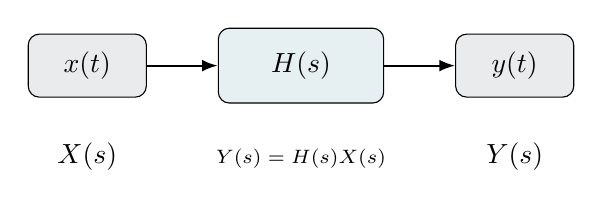
\begin{tikzpicture}[node distance=0.8cm]
          \node[draw, rounded corners, fill=PrimaryColor!10, minimum width=1.5cm, minimum height=0.8cm] (x) {$x(t)$};
          \node[draw, rounded corners, fill=AccentColor!16, minimum width=2.1cm, minimum height=0.95cm, right=0.9cm of x] (h) {$H(s)$};
          \node[draw, rounded corners, fill=PrimaryColor!10, minimum width=1.5cm, minimum height=0.8cm, right=0.9cm of h] (y) {$y(t)$};
          \draw[-{Latex[length=2mm]}, thick] (x) -- (h);
          \draw[-{Latex[length=2mm]}, thick] (h) -- (y);

          \node[below=0.45cm of x] {$X(s)$};
          \node[below=0.45cm of h] {\scriptsize $Y(s)=H(s)X(s)$};
          \node[below=0.45cm of y] {$Y(s)$};
        \end{tikzpicture}
      \end{center}

      \vspace{0.12cm}
      \begin{conceptbox}{Eigenfunction Reminder}
        For $x(t)=e^{st}$,
        \[
          y(t)=H(s)e^{st}
        \]
        whenever $s$ lies in the ROC of $H(s)$.
      \end{conceptbox}
    \end{column}
  \end{columns}
\end{frame}

\begin{frame}[t]{Causality from the ROC}
  \small
  \begin{columns}[T]
    \begin{column}{0.55\textwidth}
      \begin{conceptbox}{Causality Tests}
        \begin{itemize}
          \item If a system is causal, then $h(t)=0$ for $t<0$, so the ROC of $H(s)$ is a right-half plane.
          \item If $H(s)$ is \textbf{rational}, causality is equivalent to the ROC being to the right of the rightmost pole.
        \end{itemize}
      \end{conceptbox}

      \textbf{Example 9.17}
      \[
        h(t)=e^{-t}u(t)
        \Longrightarrow
        H(s)=\frac{1}{s+1},
        \quad \text{Re}\{s\}>-1
      \]
      Right-sided impulse response, so the system is causal.

      \vspace{0.05cm}
      \textbf{Example 9.18}
      \[
        h(t)=e^{-|t|}
        \Longrightarrow
        H(s)=\frac{-2}{s^2-1},
        \quad -1<\text{Re}\{s\}<1
      \]
      Two-sided impulse response, so the system is \textbf{not} causal.
    \end{column}
    \begin{column}{0.45\textwidth}
      \vspace{0.5cm}
      \begin{center}
        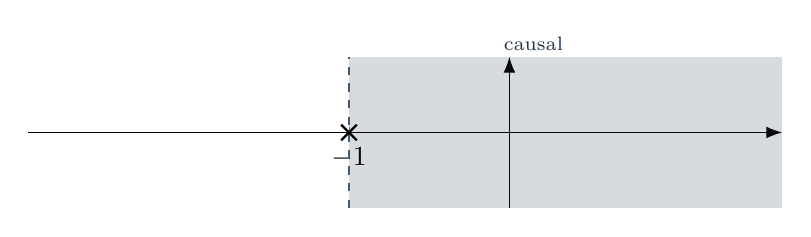
\begin{tikzpicture}
          \begin{axis}[
              width=0.92\textwidth, height=3.5cm,
              axis lines=middle, axis line style={-{Latex[length=2mm]}},
              xmin=-3, xmax=1.7, ymin=-1.7, ymax=1.7,
              xtick={-1}, xticklabels={$-1$}, ytick=\empty,
              clip=false
            ]
            \fill[PrimaryColor, fill opacity=0.18] (axis cs:-1,-1.7) rectangle (axis cs:1.7,1.7);
            \draw[dashed, thick, DarkGray] (axis cs:-1,-1.7) -- (axis cs:-1,1.7);
            \addplot[only marks, mark=x, mark options={scale=2, thick}] coordinates {(-1,0)};
            \node[PrimaryColor] at (axis cs:0.15,2) {\scriptsize causal};
          \end{axis}
        \end{tikzpicture}

        \vspace{0.5cm}
        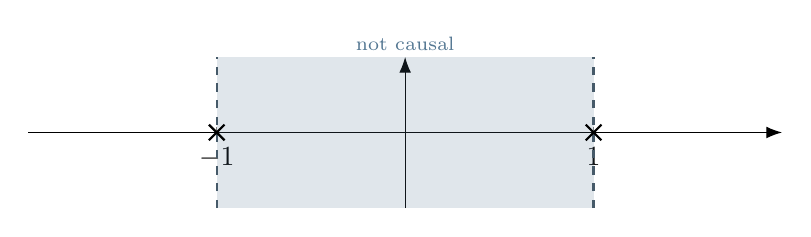
\begin{tikzpicture}
          \begin{axis}[
              width=0.92\textwidth, height=3.5cm,
              axis lines=middle, axis line style={-{Latex[length=2mm]}},
              xmin=-2, xmax=2, ymin=-1.7, ymax=1.7,
              xtick={-1,1}, xticklabels={$-1$,$1$}, ytick=\empty,
              clip=false
            ]
            \fill[SecondaryColor, fill opacity=0.18] (axis cs:-1,-1.7) rectangle (axis cs:1,1.7);
            \draw[dashed, thick, DarkGray] (axis cs:-1,-1.7) -- (axis cs:-1,1.7);
            \draw[dashed, thick, DarkGray] (axis cs:1,-1.7) -- (axis cs:1,1.7);
            \addplot[only marks, mark=x, mark options={scale=2, thick}] coordinates {(-1,0) (1,0)};
            \node[SecondaryColor] at (axis cs:0,2) {\scriptsize not causal};
          \end{axis}
        \end{tikzpicture}
      \end{center}
    \end{column}
  \end{columns}
\end{frame}

\begin{frame}[t]{Stability from the ROC: Example 9.20}
  \small
  \begin{columns}[T]
    \begin{column}{0.48\textwidth}
      \begin{conceptbox}{Stability Test}
        An LTI system is stable iff the ROC of $H(s)$ includes the entire $j\omega$-axis.
      \end{conceptbox}

      Consider
      \[
        H(s)=\frac{s-1}{(s+1)(s-2)}
      \]
      The poles are at $s=-1$ and $s=2$, so there are three possible ROCs:

      \vspace{0.1cm}
      \begin{itemize}
        \item $\text{Re}\{s\}>2$: causal, but unstable
        \item $-1<\text{Re}\{s\}<2$: noncausal, but stable
        \item $\text{Re}\{s\}<-1$: anticausal, and unstable
      \end{itemize}

      \vspace{0.1cm}
      Only the middle ROC contains the $j\omega$-axis.
    \end{column}
    \begin{column}{0.52\textwidth}
      \begin{center}
        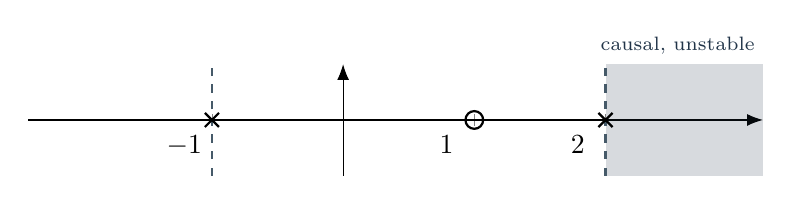
\begin{tikzpicture}
          \begin{axis}[
              width=0.9\textwidth, height=3cm,
              axis lines=middle, axis line style={-{Latex[length=2mm]}},
              xmin=-2.4, xmax=3.2, ymin=-1.5, ymax=1.5,
              xtick={-1,1,2}, xticklabels={$-1\qquad$,$1\qquad$,$2\qquad$}, ytick=\empty,
              clip=false
            ]
            \fill[PrimaryColor, fill opacity=0.18] (axis cs:2,-1.5) rectangle (axis cs:3.2,1.5);
            \draw[dashed, thick, DarkGray] (axis cs:-1,-1.5) -- (axis cs:-1,1.5);
            \draw[dashed, thick, DarkGray] (axis cs:2,-1.5) -- (axis cs:2,1.5);
            \addplot[only marks, mark=x, mark options={scale=1.8, thick}] coordinates {(-1,0) (2,0)};
            \addplot[only marks, mark=o, mark options={scale=1.6, thick}] coordinates {(1,0)};
            \node[PrimaryColor] at (axis cs:2.55,2) {\scriptsize causal, unstable};
          \end{axis}
        \end{tikzpicture}

        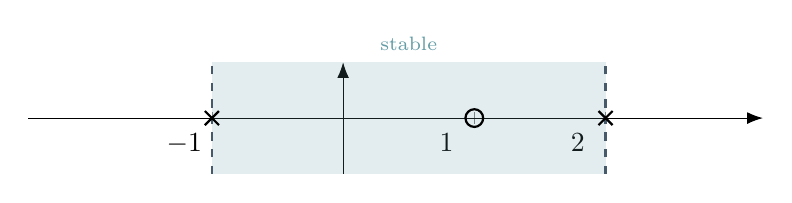
\begin{tikzpicture}
          \begin{axis}[
              width=0.9\textwidth, height=3cm,
              axis lines=middle, axis line style={-{Latex[length=2mm]}},
              xmin=-2.4, xmax=3.2, ymin=-1.5, ymax=1.5,
              xtick={-1,1,2}, xticklabels={$-1\qquad$,$1\qquad$,$2\qquad$}, ytick=\empty,
              clip=false
            ]
            \fill[AccentColor, fill opacity=0.18] (axis cs:-1,-1.5) rectangle (axis cs:2,1.5);
            \draw[dashed, thick, DarkGray] (axis cs:-1,-1.5) -- (axis cs:-1,1.5);
            \draw[dashed, thick, DarkGray] (axis cs:2,-1.5) -- (axis cs:2,1.5);
            \addplot[only marks, mark=x, mark options={scale=1.8, thick}] coordinates {(-1,0) (2,0)};
            \addplot[only marks, mark=o, mark options={scale=1.6, thick}] coordinates {(1,0)};
            \node[AccentColor] at (axis cs:0.5,2) {\scriptsize stable};
          \end{axis}
        \end{tikzpicture}

        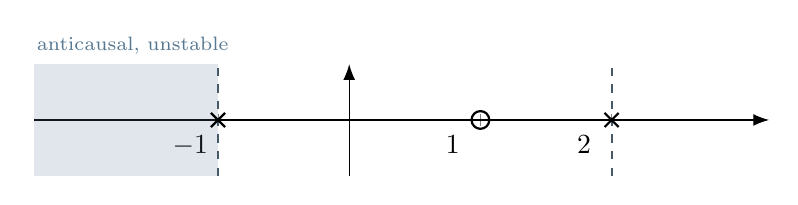
\begin{tikzpicture}
          \begin{axis}[
              width=0.9\textwidth, height=3cm,
              axis lines=middle, axis line style={-{Latex[length=2mm]}},
              xmin=-2.4, xmax=3.2, ymin=-1.5, ymax=1.5,
              xtick={-1,1,2}, xticklabels={$-1\qquad$,$1\qquad$,$2\qquad$}, ytick=\empty,
              clip=false
            ]
            \fill[SecondaryColor, fill opacity=0.18] (axis cs:-2.4,-1.5) rectangle (axis cs:-1,1.5);
            \draw[dashed, thick, DarkGray] (axis cs:-1,-1.5) -- (axis cs:-1,1.5);
            \draw[dashed, thick, DarkGray] (axis cs:2,-1.5) -- (axis cs:2,1.5);
            \addplot[only marks, mark=x, mark options={scale=1.8, thick}] coordinates {(-1,0) (2,0)};
            \addplot[only marks, mark=o, mark options={scale=1.6, thick}] coordinates {(1,0)};
            \node[SecondaryColor] at (axis cs:-1.65,2) {\scriptsize anticausal, unstable};
          \end{axis}
        \end{tikzpicture}
      \end{center}
    \end{column}
  \end{columns}
\end{frame}

\begin{frame}[t]{Rational Causal Stability and Pole Locations}
  \small
  \begin{columns}[T]
    \begin{column}{0.54\textwidth}
      \begin{conceptbox}{Pole Test for Rational Causal Systems}
        A causal system with rational $H(s)$ is stable iff all poles of $H(s)$ lie in the left half-plane.
      \end{conceptbox}

      \textbf{Example 9.21}
      \[
        H(s)=\frac{1}{s-2},
        \qquad \text{ROC}:\ \text{Re}\{s\}>2
      \]
      The ROC is causal, but the pole is at $s=2$ in the right half-plane, so the system is unstable.

    \end{column}
    \begin{column}{0.46\textwidth}
      \textbf{Fig. 9.26: Unstable Causal Second-Order}\\[0.1cm]
      \begin{center}
        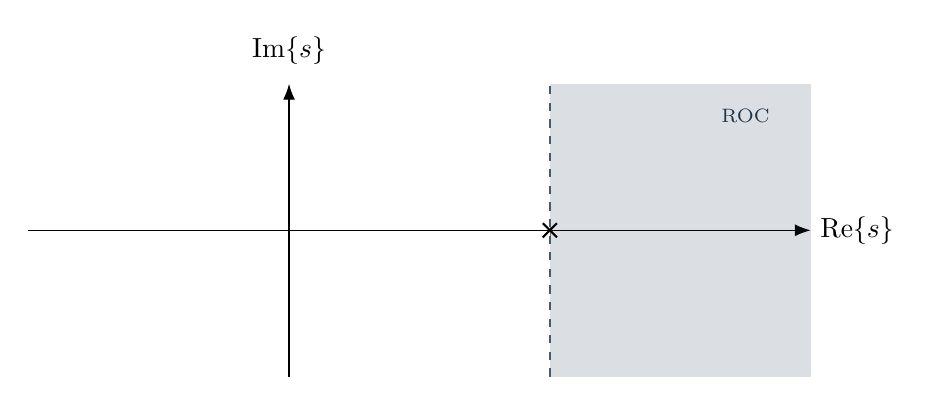
\begin{tikzpicture}
          \begin{axis}[
              width=0.95\textwidth, height=5.3cm,
              axis lines=middle, axis line style={-{Latex[length=2mm]}},
              xmin=-2, xmax=4, ymin=-2.3, ymax=2.3,
              xlabel={$\text{Re}\{s\}$},
              ylabel={$\text{Im}\{s\}$},
              xtick={2}, xticklabels={}, ytick=\empty,
              xlabel style={anchor=west, at={(axis cs:4,0)}},
              ylabel style={anchor=south, at={(axis cs:0,2.45)}},
              clip=false
            ]
            \fill[PrimaryColor, fill opacity=0.16] (axis cs:2,-2.3) rectangle (axis cs:4,2.3);
            \draw[dashed, thick, DarkGray] (axis cs:2,-2.3) -- (axis cs:2,2.3);
            \addplot[only marks, mark=x, mark options={scale=1.8, thick}] coordinates {(2,0)};
            \node[PrimaryColor] at (axis cs:3.5,1.8) {\scriptsize ROC};
          \end{axis}
        \end{tikzpicture}
      \end{center}
    \end{column}
  \end{columns}
\end{frame}

\section{Differential Equations}

\begin{frame}[t]{Obtain the System Function from a Differential Equation}
  \small
  \begin{itemize}
    \item Instead of starting with a given impulse response $h(t)$, we often are given a differential equation that describes the system.
    \item From the DE, we can find the quotient $\frac{Y(s)}{X(s)}$ of the output and input transforms.
    \item For example, if the DE is
      \[
        \frac{dy(t)}{dt}+3y(t)=x(t) \stackrel{\mathcal{L}}{\longleftrightarrow} sY(s)+3Y(s)=X(s)
      \]
      then
      \[
        \frac{Y(s)}{X(s)}=\frac{1}{s+3}
      \]
    \item Remember $H(s) = \frac{Y(s)}{X(s)}$ is the system function, so we have obtained $H(s)$ from the DE.
    \item Thus,
      \[
        H(s) = \frac{1}{s+3}
      \]
      and we can analyze the system using $H(s)$.
    \item We can also find the impulse response $h(t)$ by taking the inverse Laplace transform of $H(s)$, but we need to be careful about the ROC.
  \end{itemize}
\end{frame}

\begin{frame}[t]{Example 9.23: Obtain the System Function from a Differential Equation}
  \small
  \begin{columns}[T]
    \begin{column}{0.58\textwidth}
      Consider the system again
      \[
        \frac{dy(t)}{dt}+3y(t)=x(t)
      \]
      Taking Laplace transforms under zero initial conditions:
      \[
        sY(s)+3Y(s)=X(s)
      \]
      Hence
      \[
        H(s)=\frac{Y(s)}{X(s)}=\frac{1}{s+3}
      \]

      \vspace{0.15cm}
      \textbf{Two possible impulse responses}
      \[
        h(t)=e^{-3t}u(t), \quad \text{Re}\{s\}>-3
      \]
      or
      \[
        h(t)=-e^{-3t}u(-t), \quad \text{Re}\{s\}<-3
      \]
      The DE fixes the algebraic form; causality selects the ROC.
    \end{column}
    \begin{column}{0.42\textwidth}
      \begin{center}
        \vspace{0.25cm}

        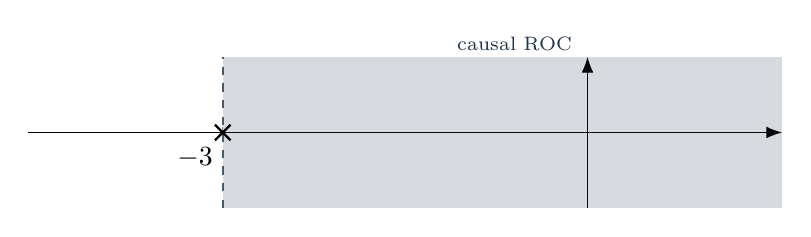
\begin{tikzpicture}
          \begin{axis}[
              width=0.92\textwidth, height=3.5cm,
              axis lines=middle, axis line style={-{Latex[length=2mm]}},
              xmin=-4.6, xmax=1.6, ymin=-1.7, ymax=1.7,
              xtick={-3}, xticklabels={$-3\qquad$}, ytick=\empty,
              clip=false
            ]
            \fill[PrimaryColor, fill opacity=0.18] (axis cs:-3,-1.7) rectangle (axis cs:1.6,1.7);
            \draw[dashed, thick, DarkGray] (axis cs:-3,-1.7) -- (axis cs:-3,1.7);
            \addplot[only marks, mark=x, mark options={scale=2, thick}] coordinates {(-3,0)};
            \node[PrimaryColor] at (axis cs:-0.6,2) {\scriptsize causal ROC};
          \end{axis}
        \end{tikzpicture}

        \vspace{0.5cm}
        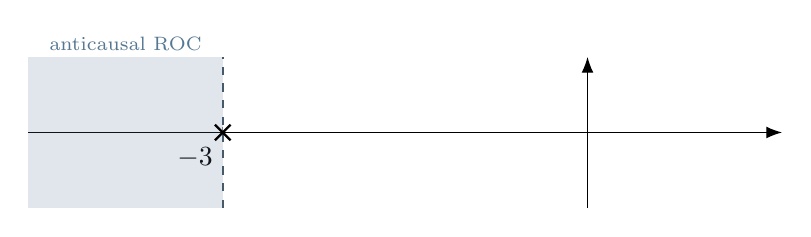
\begin{tikzpicture}
          \begin{axis}[
              width=0.92\textwidth, height=3.5cm,
              axis lines=middle, axis line style={-{Latex[length=2mm]}},
              xmin=-4.6, xmax=1.6, ymin=-1.7, ymax=1.7,
              xtick={-3}, xticklabels={$-3\qquad$}, ytick=\empty,
              clip=false
            ]
            \fill[SecondaryColor, fill opacity=0.18] (axis cs:-4.6,-1.7) rectangle (axis cs:-3,1.7);
            \draw[dashed, thick, DarkGray] (axis cs:-3,-1.7) -- (axis cs:-3,1.7);
            \addplot[only marks, mark=x, mark options={scale=2, thick}] coordinates {(-3,0)};
            \node[SecondaryColor] at (axis cs:-3.8,2) {\scriptsize anticausal ROC};
          \end{axis}
        \end{tikzpicture}
      \end{center}
    \end{column}
  \end{columns}
\end{frame}

\begin{frame}[t]{Solving a Differential Equation with LT}
  \small
  \begin{columns}[T]
    \begin{column}{0.58\textwidth}
      Use the causal system from Example 9.23:
      \[
        H(s)=\frac{1}{s+3},
        \qquad h(t)=e^{-3t}u(t)
      \]
      Let the input be
      \[
        x(t)=e^{-2t}u(t)
        \Longleftrightarrow
        X(s)=\frac{1}{s+2}
      \]
      Then
      \[
        Y(s)=H(s)X(s)=\frac{1}{(s+2)(s+3)}
      \]
      Partial fractions give
      \[
        Y(s)=\frac{1}{s+2}-\frac{1}{s+3}
      \]
      so
      \[
        y(t)=\left(e^{-2t}-e^{-3t}\right)u(t)
      \]
      The transform method solved the DE by turning it into algebra and then using known inverse LT pairs.
    \end{column}
    \begin{column}{0.42\textwidth}
      \begin{conceptbox}{System Classification}
        \begin{itemize}
          \item Pole at $s=-3$
          \item ROC is $\text{Re}\{s\}>-3$
          \item Causal: \cmark
          \item Stable: \cmark
        \end{itemize}
      \end{conceptbox}

      \vspace{0.15cm}
      \begin{center}
        \begin{tikzpicture}
          \begin{axis}[
              width=0.92\textwidth, height=3.8cm,
              axis lines=middle, axis line style={-{Latex[length=2mm]}},
              xmin=-0.3, xmax=4.3, ymin=-0.05, ymax=0.35,
              xtick={0}, ytick={0.3},
              yticklabels={$0.3$},
              xlabel={$t$}, ylabel={$y(t)$},
              xlabel style={anchor=west, at={(axis cs:4.35,0)}},
              ylabel style={anchor=south, at={(axis cs:0,0.37)}},
              declare function={resp(\t) = \t >= 0 ? exp(-2*\t) - exp(-3*\t) : 0;},
              clip=false
            ]
            \addplot[thick, PrimaryColor, domain=-0.3:4.3, samples=200] {resp(x)};
          \end{axis}
        \end{tikzpicture}
      \end{center}
    \end{column}
  \end{columns}
\end{frame}

\begin{frame}[t]{LCCDEs Become Algebra in the Laplace Domain}
  \small
  \begin{columns}[T]
    \begin{column}{0.57\textwidth}
      Suppose the input and output satisfy the linear constant-coefficient differential equation
      \[
        \sum_{k=0}^{N} a_k \frac{d^k y(t)}{dt^k}
        =
        \sum_{k=0}^{M} b_k \frac{d^k x(t)}{dt^k}
      \]
      Under zero initial conditions, the differentiation property gives
      \[
        \left(\sum_{k=0}^{N} a_k s^k\right)Y(s)
        =
        \left(\sum_{k=0}^{M} b_k s^k\right)X(s)
      \]

      \begin{conceptbox}{System Function from an LCCDE}
        \[
          H(s) \triangleq \frac{Y(s)}{X(s)}
          =
          \frac{\sum_{k=0}^{M} b_k s^k}{\sum_{k=0}^{N} a_k s^k}
        \]
      \end{conceptbox}

      Zeros come from the numerator, poles from the denominator, and the ROC still depends on causality or other side information.
    \end{column}
    \begin{column}{0.43\textwidth}
      \begin{center}
        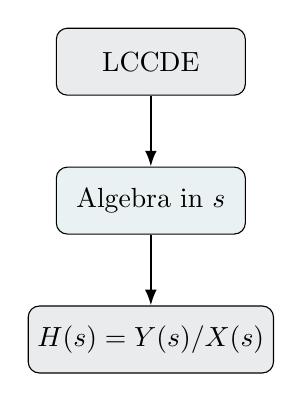
\begin{tikzpicture}[node distance=0.95cm]
          \node[draw, rounded corners, fill=PrimaryColor!10, minimum width=2.4cm, minimum height=0.85cm] (de) {LCCDE};
          \node[draw, rounded corners, fill=AccentColor!14, minimum width=2.4cm, minimum height=0.85cm, below=0.9cm of de] (alg) {Algebra in $s$};
          \node[draw, rounded corners, fill=PrimaryColor!10, minimum width=2.8cm, minimum height=0.85cm, below=0.9cm of alg] (hs) {$H(s)=Y(s)/X(s)$};
          \draw[-{Latex[length=2mm]}, thick] (de) -- (alg);
          \draw[-{Latex[length=2mm]}, thick] (alg) -- (hs);
        \end{tikzpicture}
      \end{center}

      \vspace{0.15cm}
      A differential equation in time becomes a polynomial ratio in $s$, which makes solving and classifying systems much easier.
    \end{column}
  \end{columns}
\end{frame}

\end{document}
